
%% bare_conf.tex
%% V1.3
%% 2007/01/11
%% by Michael Shell
%% See:
%% http://www.michaelshell.org/
%% for current contact information.
%%
%% This is a skeleton file demonstrating the use of IEEEtran.cls
%% (requires IEEEtran.cls version 1.7 or later) with an IEEE conference paper.
%%
%% Support sites:
%% http://www.michaelshell.org/tex/ieeetran/
%% http://www.ctan.org/tex-archive/macros/latex/contrib/IEEEtran/
%% and
%% http://www.ieee.org/


\documentclass[conference]{IEEEtran}
\usepackage{blindtext, graphicx}
\usepackage[justification=centering]{caption}
\usepackage[utf8]{inputenc}
\usepackage[T1]{fontenc}
\usepackage[english,portuguese]{babel}
\usepackage{hyphenat}
\hyphenation{mate-mática recu-perar}
\hyphenation{op-tical net-works semi-conduc-tor}
\usepackage{verbatim}
\usepackage{color}


\begin{document}

%\title{Identificação e Rastreamento de Pessoas em Ambientes Internos Utilizando Humanos Como Sensores}
\title{Utilizando Mapas de Profundidade para Detecção de Pessoas em Ambientes Internos}

\author{
\IEEEauthorblockN{Edivaldo M. F. de Jesus Jr.}
\IEEEauthorblockA{Especialização em Computação Distribuída e Ubíqua\\
Grupo de Sistemas Distribuídos, Otimização, Redes e \\
Tempo-Real - GSORT\\
edivaldojunior@ifba.edu.br}

\and
\IEEEauthorblockN{Manoel C. M. Neto}
\IEEEauthorblockA{Especialização em Computação Distribuída e Ubíqua\\
Grupo de Sistemas Distribuídos, Otimização, Redes e \\
Tempo-Real - GSORT\\
manoelnetom@ifba.edu.br}
}

\maketitle

{\selectlanguage{english}
\begin{abstract}
The Advancement of location technologies has been providing grants for creating efficient and robust applications. Due to the fact that people spend most of their time in indoors environments, these indoor tracking services are in great demand from the public. Although various approaches have been proposed to deal with this problem, solutions still remain untackled due to various reasons (e.g. user acceptance). Based on this observation, this paper aims to provide a better understanding of the technologies currently used and stimulate a recent concept in sensory area: using depth maps generated by Microsoft Kinect for this purpose.
\end{abstract}}

\begin{abstract}
O avanço nas tecnologias de localização tem fornecido subsídios para criação de aplicações eficientes e robustas. Devido ao fato de que as pessoas passam a maior parte do seu tempo em ambientes fechados, serviços de detecção e rastreamento estão em grande demanda do público. Embora tenham sido propostas várias abordagens para lidar com este problema, as soluções ainda permanecem não resolvidas. Problemas como pose, iluminação e aceitação do usuário são alguns dos desafios complexos para o reconhecimento de faces 2D. Com base nessa observação, este trabalho tem como objetivo proporcionar uma melhor compreensão das tecnologias atualmente utilizadas e estimular um recente conceito na área sensorial: a utilização de mapas de profundidade. Menos intrusivo, se comparado à soluções com cameras RGB e custos muito abaixo dos scanners 3D tradicionais, o Microsoft Kinect é capaz de fornecer esse mapa de profundidade que é entao processado por um algoritmo e, em caso de detecção, os dados são exportados para que plataformas externas possam consumí-los. Dados obtidos foram comparados com outros mecanismos de detecção, e os resultados apresentados.  
\end{abstract}

{\selectlanguage{portuguese}
\begin{IEEEkeywords}
Detecção de pessoas, localização, ambientes internos.
\end{IEEEkeywords}}

\IEEEpeerreviewmaketitle


%Seções
\section{Introdução}\label{sec:introducao}

Detecção e rastreamento de pessoas são problemas desafiadores, especialmente em cenários reais e complexos. Esses cenários normalmente envolvem várias pessoas, obstruções e origens desordenadas ou ainda cenários com plano de fundo em movimento. Detectores de pessoas têm se mostrado capazes de localizar os pedestres mesmo em cenas complexas de rua. Entretanto, falsos positivos são frequentemente encontrados \cite{andriluka2008people}. A identificação de indivíduos particulares permanece igualmente desafiadora.
Métodos de rastreamento são capazes de encontrar um indivíduo em particular em sequências de imagens, mas são severamente desafiados por cenários do mundo real, tais como cenas de uma rua lotada \cite{andriluka2008people}.

Para ambientes abertos, sistemas de GPS (\textit{Global Positioning System}) desempenham um papel dominante no que se refere à localização \cite{fritsche2009}. No entanto, essa tecnologia não funciona bem em ambientes fechados. Essa ineficiência é consequência da fraqueza de sinais emitidos por GPS e a sua incapacidade de penetrar a maioria dos materiais de construção. Portanto, GPS não se encaixa bem em ambientes internos onde as pessoas passam a maior parte do seu tempo. Mesmo que os dispositivos GPS se tornem mais promissores e ponderáveis no futuro, sendo capazes de proporcionar uma precisão suficiente para uso ao ar livre, tecnologias mais eficazes são exigidas para o rastreamento de humanos e objetos em ambientes interiores \cite{zhang2010localization}.

Devido à complexidade desses ambientes, o desenvolvimento de uma técnica de localização interna é sempre acompanhado de um conjunto de desafios, como por exemplo: objetos fora do ângulo de visão (\textit{non line of sight} - NLOS); efeito de caminhos múltiplos; e interferência de ruído. Esses desafios resultam principalmente da influência de obstáculos (paredes, equipamentos, e/ou seres humanos) na propagação de ondas eletromagnéticas. A mobilidade das pessoas incorre mudanças nas condições físicas do ambiente, o que pode afetar de forma significativa o comportamento da propagação de sinal \textit{wireless}, por exemplo \cite{zhang2010localization}. 

Um sistema de localização interior, como definido por Dempsey \cite{dempsey2003indoor}, é um sistema que pode determinar a posição de algo ou alguém em um espaço físico, como em um hospital, um ginásio, uma escola, etc., de forma contínua e em tempo real. Porém, rastrear e acompanhar o movimento de pessoas em ambientes internos é útil para uma variedade de aplicações, incluindo cuidados a bebês e idosos, estudo do comportamento do cliente nos \textit{shopping centers}, segurança, etc. \cite{yiu2007tracking}.

Sensores de infravermelho passivos (PIR- \textit{Passive infrared}) são comumente usados em conjunto com uma variedade de outros sensores em diversas aplicações para a construção de ambientes inteligentes, como saúde, sistema de energia inteligente e segurança \cite{yun2014human}.

O conceito de Casa inteligente (\textit{Smart Home}) compreende vários serviços associados para cumprir objetivos diferentes. Sua finalidade é reforçar as atividades rotineiras dos habitantes, facilitando a vida independente de pessoas com deficiência, pacientes e idosos residentes \cite{al2014advanced}. Esses serviços podem ser divididos em seis categorias: conforto, gestão de energia, multimídia e entretenimento, saúde, segurança e proteção, e comunicações \cite{dewsbury2001process}.

Porém, criar uma abordagem de detecção e identificação humana é um problema desafiador, devido à complexidade das condições ambientais de espaços inteligentes e a variedade de serviços e demandas dos usuários \cite{al2014advanced}.

O processo de localização inteiro é dividido em duas fases: a medição de sinal e de cálculo de posição \cite{zhang2010localization}. 

Nos últimos anos vários métodos foram propostos para detecção humana \cite{dalal2005,dalal2006,ikemura2011,schwartz2009}. A maior parte da pesquisa é feita baseada em imagens extraídas de câmeras de luz visível (Câmeras RGB), que é uma maneira natural de fazê-la, exatamente como os olhos humanos funcionam. Alguns métodos envolvem o treino estatístico com base em características locais, tais como Histograma de Gradiente Orientado (\textit{Histograms of Oriented gradient} – HOG) \cite{dalal2005}., Histogramas de Orientação de Borda (\textit{Edge Orientation Histograms} – EOH) \cite{levi2004}, e alguns envolvem a extração de pontos de interesse na imagem, tais como transformada de característica invariante em escala (\textit{Scale-invariant Feature Transform} - SIFT) \cite{lowe1999}, etc.

Embora muitos relatórios tenham mostrado que esses métodos podem fornecer resultados de detecção altamente precisos, os métodos baseados em imagens RGB encontram dificuldades em perceber as formas dos sujeitos com poses articuladas ou quando o plano de fundo está incompreensível \cite{xia2011human}. Isso resultará na queda da precisão ou no aumento do custo computacional. As informações de profundidade são uma sugestão importante quando o ser humano reconhece objetos porque os objetos podem não ter cor e textura consistentes, mas devem ocupar uma região integrada no espaço \cite{xia2011human}. 

É notavelmente crescente nas últimas décadas pesquisas utilizando imagem de profundidade para o reconhecimento ou modelagem de objetos \cite{sabata1993, vemuri1986}. As imagens de profundidade têm várias vantagens sobre as imagens de intensidade 2D, dentre elas: as imagens de profundidade são resistentes à mudança de cor e de iluminação. Além disso, as imagens de alcance são representações simples de informações 3D. Contudo, os sensores de alcance de profundidade são caros e difíceis de utilizar em ambientes habitados devido à utilização de lasers. Uma alternativa é a utilização do Microsoft Kinect, o qual além de ser mais barato e fácil de usar, se comparado aos scanners 3D convencionais, não tem as desvantagens da utilização de laser\cite{xia2011human}.

Apesar do grande progresso nos últimos anos, há uma série de questões em aberto que precisam ser abordadas. Exemplos incluem rastreamento contínuo de pessoas que circulam entre ambientes internos e externos, a resolução de problemas de sincronização, reduzindo o impacto da interferência de ruído e melhorar a eficiência energética. Embora algumas tecnologias anteriores estejam preocupados com estas questões, elas podem sofrer de várias limitações, por exemplo, em aumentar o custo de todo o sistema, a deficiência de precisão, e sobrecarga computacional \cite{zhang2010localization}.

Este trabalho utiliza mapas de profundidade gerados pelo Kinect com o objetivo de detectar pessoas em um ambiente fechado.

Além desta Introdução, este trabalho está estruturado da seguinte forma:
A Seção \ref{sec:referencial-teorico} apresenta várias tecnologias envolvidas na preparação deste trabalho. A Seção \ref{sec:trabalhos-relacionados} apresenta os trabalhos correlatos. A Seção \ref{sec:solucao-desenvolvida} apresenta detalhes da implementação a ser desenvolvida. A Seção \ref{sec:conclusao} conclui este trabalho, destacando as suas limitações e trabalhos futuros.
\section{Referencial Teórico}\label{sec:referencial-teorico}

Nesta Seção, os principais conceitos relacionados a este trabalho são apresentados, fornecendo subsídios para o desenvolvimento do projeto de detecção de pessoas em ambiente fechado, usando mapas de profundidade. A subseção \ref{sec:biometria} expõe informações referentes à biometria e sistemas biométricos. A subseção \ref{sec:deteccao-rastreamento} apresenta conceitos relacionados à detecção e rastreamento de pessoas. A subseção \ref{sec:tec-rastreamento} discute o tópico tecnologias de rastreamento. Na subseção \ref{sec:determ-posic} são abordadas as técnicas de determinação de posição comumente utilizadas. A subseção \ref{sec:recFacial} explicita a definição de reconhecimento facial. Por fim, na subseção \ref{sec:kinect} são apresentadas informações e conceitos referentes ao \textit{Microsoft Kinect}.

\subsection{Biometria e Sistemas Biométricos}\label{sec:biometria}
O termo biometria deriva do grego bios (vida) + metron (medida) e, na autenticação, refere-se à utilização de características próprias de um indivíduo para proceder à sua autenticação e/ou identificação \cite{magalhaes2003biometria}. Na biometria utiliza-se características físicas/fisiológicas ou comportamentais para a identificação de pessoas, sendo baseada em algo que a pessoa e e não em algo que ela possui ou sabe. A Figura~\ref{fig:biometria} ilustra exemplos de características biométricas \cite{cardia2015avaliaccao}.

\begin{figure*}[ht]
\centering
    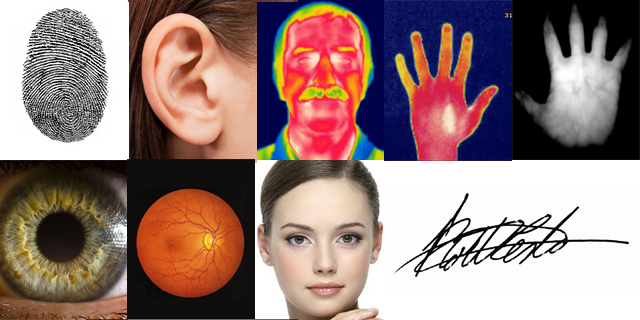
\includegraphics[resolution=300,width=0.7\textwidth,natwidth=610,natheight=642]{images/biometria.png}
    \caption{Exemplos de características biométricas: impressão digital, orelha, termograma facial, termograma da mão, padrões de veias da mão, íris, retina, face e assinatura.}
    \label{fig:biometria}
\end{figure*}

Características físicas/fisiológicas são baseadas na anatomia ou no funcionamento do organismo de uma pessoa viva, como impressão digital ou termograma facial. Já as comportamentais são baseadas na forma particular que um sujeito executa uma ação, como o a dinâmica de digitação ou a assinatura captada de modo digital. Qualquer característica pode ser utilizada desde que atenda algumas restrições, tais como \cite{maltoni2009handbook}:

\begin{itemize}
\item Universalidade: A característica deve estar presente na maior quantidade possível de pessoas;
\item Unicidade: A característica deve ser diferente entre pessoas diferentes;
\item Permanência: A característica não deve mudar com o passar do tempo;
\item Mensurabilidade: A característica deve ser fácil de coletar e mensurar;
\item Desempenho: A característica deve permitir alta acurácia com baixo tempo de processamento e custo computacional, além de ser robusta a ambientes não controlados;
\item Aceitabilidade: A característica deve ser aceita facilmente pelas pessoas como forma de identificação;
\item Grau de impostura: A característica deve ser resistente a fraude.
\end{itemize}

Um sistema de reconhecimento de padrões que utiliza um vetor de característica baseado em qualquer traço biométrico para garantir a identidade de uma pessoa é um sistema biométrico. Esses sistemas recebem a característica da pessoa, e processa em uma forma reduzida chamada de \textit{template}. Esse \textit{template} pode ser armazenado em um banco de dados central ou em um dispositivo de mídia removível. Segundo Wayman \cite{wayman2002}, um sistema biométrico pode ser classificado em uma das setes categorias: 

\begin{itemize}
\item Cooperativo ou não cooperativo: O sujeito deseja ser identificado?
\item Evidente ou sigiloso: O sujeito sabe que ele está sendo identificado?
\item Habituado ou não habituado: O sujeito frequentemente se submete a identificação?
\item Auxiliado ou não auxiliado: Existe um operador humano auxiliando o sistema?
\item Ambiente controlado ou não controlado: Em qual ambiente o sistema irá operar?
\item Privado ou público: Os sujeitos são empregados (privado) ou clientes (público)?
\item Aberto ou fechado: O sistema precisa de padrões para ter interoperabilidade entre sistemas?
\end{itemize}




\subsection{Detecção, identificação e rastreamento}\label{sec:deteccao-rastreamento}

As aplicações de localização interior têm experimentado esforços adicionais nos últimos anos com o aparecimento da computação ubíqua. Em vários cenários, objetos e mercadorias devem estar localizados ou monitorados, por exemplo, em um ambiente industrial ou médico. Adicionalmente, a localização de pessoas permite a criação de uma série de aplicativos e serviços. Clientes e funcionários podem ser observados, invasores detectados, idosos assistidos, e pacientes acompanhados. Em locais públicos, como estações de metrô, as preocupações de segurança podem ser abordadas por um sistema de orientação de emergência \cite{linde2006aspects}. 

Segundo Jaeseok Yun e Sang-Shin Lee \cite{yun2014human}, um sistema de controle de movimentos deve detectar robustamente: 
\begin{itemize}
  \item A identidade do objeto em movimento;
  \item Em qual o local está o objeto; 
  \item Em que sentido o objeto está se movimentando;
  \item O quão rápido esse objeto se move. 
 \end{itemize}

Uma das questões-chave da emergente computação móvel e robótica é a obtenção do conhecimento da posição de pessoas e objetos em um ambiente interno \cite{linde2006aspects}. A fim de construir um ambiente inteligente, onde os sistemas possam entender as atividades nas quais o usuário está envolvido e suas imediações, para então adaptar os seus serviços e recursos para o contexto do usuário, é necessário desenvolver um sistema de detecção, identificação e rastreamento de movimento robusto usando vários sensores \cite{yun2014human}. Esses três conceitos serão discutidos a seguir.


\subsubsection{Detecção de pessoas}\label{sec:deteccao-movimento}
Detectar seres humanos em imagens é uma tarefa desafiadora devido à sua aparência variável e à ampla gama de poses que eles podem adotar. A primeira necessidade é um conjunto de características robustas que permite que a forma humana seja discriminada de forma limpa, mesmo em ambientes despropositados sob iluminação difícil. Estudada a questão dos conjuntos de recursos para a detecção humana, dentre os principais métodos está  os descritores de histograma de desdobramento orientado (HOG) \cite{dalal2005histograms}. Os recursos baseados em gradientes, como HOG e EOH, envolvem a extração de pontos de interesse na imagem, como transformação de característica invariante em escala (EIPD), etc. Embora muitos relatórios mostrem que esses métodos possam fornecer resultados de detecção de humanos altamente precisos, os métodos baseados em imagem RGB encontram dificuldades em perceber as formas dos seres humanos com poses articuladas ou quando o fundo é confuso. Isso resulta na diminuição da precisão ou no aumento do custo computacional\cite{dalal2005histograms}.

\subsubsection{Identificação de indivíduos}\label{sec:identificacao-pessoas}

Sistemas de sensores para identificação recolhem um conjunto de dados brutos do corpo humano, bem como extraem características distintas visando reconhecer o contexto principal: a identidade do objeto \cite{yun2014human}. Para esse fim, inúmeros sistemas têm sido estudados usando vários sensores, incluindo câmeras, sensores de movimento, blocos de pressão, radares, sensores de campo elétrico, etc.

O termo identificação significa o ato ou processo de estabelecer a identidade, ou reconhecer, ou ainda tratar uma coisa como idêntica a outra. Significa ainda o ato, ou processo, de fazer, representar ser, ou considerar ou tratar como o mesmo ou idêntico\cite{yun2014human} .

\subsubsection{Rastreamento de pessoas}\label{sec:rastre-amb-fec}

O acompanhamento do movimento das pessoas está se tornando importante em várias áreas de aplicação, onde a atividade dos indivíduos precisam ser analisadas ou monitoradas. Em tais aplicações, uma grande quantidade de informações pode ser obtida a partir de trajetórias que dão as coordenadas espaço-temporais de cada indivíduo no meio ambiente. As informações que podem ser obtidas a partir de tais trajetórias e incluem uma contagem dinâmica do número de pessoas dentro de uma área monitorada, o tempo gasto por indivíduos em uma área e padrões de fluxo de tráfego em um ambiente \cite{segen1996camera}. 

\subsection{Tecnologias de detecção Visuais, não visuais e combinadas}\label{sec:tec-rastreamento}
No geral, sistemas de monitoramento podem ser não visuais, visuais (com ou sem a utilização de marcadores) ou uma combinação de ambos \cite{zhou2008human}.

\subsubsection{Tecnologias visuais}\label{sec:sens-genericos}
Muitos pesquisadores têm dedicado os seus esforços para a construção de sistemas de detecção de movimento robustos usando sensores baseados na visão usando câmeras. Os projetos de investigação que utilizam sensores baseados em visão consideram, principalmente, posição, velocidade, direção, forma e tamanho (ou seja, o número de \textit{pixels} em câmeras) como o contexto principal para identificar os usuários e compreender as suas atividades \cite{stauffer200l}.

Existem duas principais técnicas no acompanhamento visual do movimento humano: rastreamento baseado marcador e rastreamento livre de marcador \cite{YTao2010}.

Rastreamento visual com marcador base (\textit{Visual marker based tracking}) é uma técnica onde as câmeras são utilizadas para controlar os movimentos humanos. São adicionados identificadores sobre o corpo humano. Devido ao fato de o esqueleto humano ser uma estrutura altamente articulada, torções e rotações podem gerar movimento muito complexos. Como consequência, cada parte do corpo realiza uma trajetória de movimento imprevisível e complicada, o que pode levar a estimativa de movimento inconsistente e pouco confiável. Além disso, cenas desordenadas, ou variação de iluminação podem distrair a atenção visual a partir da posição real de um marcador. Como uma solução para esses problemas, o rastreamento visual com marcador base é preferível nestas circunstâncias \cite{zhang2002visual}.

Sistemas de rastreamento baseado em marcador visual, são bastante utilizados como um "padrão" na análise de movimento humano devido à sua informação de posição precisa (os erros são de cerca de 1mm) \cite{zhang2002visual}. Esta função de precisão otimistamente motiva aplicações populares dos sistemas de rastreamento de marcadores visuais em medicina. Por exemplo, um Sistema de Captura de Movimento foi utilizado em um estudo para avaliar a relação entre os movimentos de equilíbrio corporal e as características antropométricas dos indivíduos, enquanto eles estavam em duas pernas com os olhos abertos e fechados \cite{kejonen2003}.

Entretanto, essas tecnologias possuem limitações as quais podem apresentar falhas devido:

\begin{enumerate}
    \item A identificação dos pontos ósseos padrões pode não ser confiável; 
    \item O tecido macio que se sobrepõe pontos ósseos podem mover-se, dando origem a dados ruidosos; 
    \item O próprio marcador pode oscilar devido à sua própria inércia; 
    \item Marcadores podem mesmo vir à deriva completamente.
\end{enumerate}

Sistemas visuais de rastreamento livres de marcador (\textit{Marker-free visual based tracking systems}) somente exploram sensores óticos para medir o movimentos do corpo humano. Esta aplicação é motivada pelas falhas do uso de sistemas baseados em marcador visual, anteriormente apresentadas. Como uma técnica de captura de movimento menos restritiva, os sistemas sem marcador são capazes de superar o problema de oclusão mútua, por exemplo, uma vez que se preocupam principalmente com os limites ou características dos corpos humanos\cite{zhou2008human}.

Câmeras mais avançadas podem fornecer uma resolução de um milhão de \textit{pixels}, indicando uma alta precisão na detecção de movimentos de objetos. Além disso, as câmeras hoje em dia podem ser facilmente obtidas com um baixo custo, e os parâmetros podem ser configurados de forma flexível pelo usuário. Esses méritos incentivam as filmadoras a serem usadas popularmente em aplicações de vigilância. O \textit{trade-off} se dá pelo fato de que esta técnica requer uma computação intensiva para realizar a localização 3D e a redução de erros, além da minimização da latência dos dados \cite{bryson1993}. Além disso, são necessárias câmeras de alta velocidade, já que as câmeras convencionais (com uma taxa de amostragem inferior a sessenta quadros por segundo) fornecem uma largura de banda insuficiente para uma representação de dados precisa \cite{bhatnagar1993position}.


\begin{table*}[ht]
\centering
\caption{Exemplos de aplicações que utilizam localização interna \cite{linde2006aspects}.}
\label{table:aplicacoes}
\begin{tabular}[ht]{llllllllp{2.5cm}p{8cm}}
\begin{sideways}Indústria \end{sideways} & \begin{sideways}Logística\end{sideways} & \begin{sideways}Comercial\end{sideways} & \begin{sideways}Médico\end{sideways} & \begin{sideways}Casas Inteligentes\end{sideways} & \begin{sideways}Lugares Públicos \end{sideways}& \begin{sideways}Turismo\end{sideways} & \begin{sideways}Redes de sensores\end{sideways} & Objetivo   & Propósito \\  \hline
$\boxtimes$ & $\boxtimes$ & $\Box$      & $\Box$      & $\Box$      & $\Box$      & $\Box$      & $\Box$      & Veículos guiados e robôs   & Navegação na unidade de produção ou armazém \\
$\boxtimes$ & $\boxtimes$ & $\boxtimes$ & $\boxtimes$ & $\boxtimes$ & $\Box$      & $\Box$      & $\Box$      & produtos   & Encontrar bens / objetos           \\
$\Box$      & $\Box$      & $\boxtimes$ & $\Box$      & $\Box$      & $\Box$      & $\Box$      & $\Box$      & Clientes   & Perfis dos hábitos dos clientes, assistente de compras pela navegação          \\
$\Box$      & $\Box$      & $\Box$      & $\Box$      & $\boxtimes$ & $\Box$      & $\Box$      & $\Box$      & Pessoas    & Controle climático da casa inteligente, características de conveniência, detecção de intruso, monitoramento eletrônico de prisão domiciliar          \\
$\Box$      & $\Box$      & $\Box$      & $\boxtimes$ & $\Box$      & $\Box$      & $\Box$      & $\Box$      & Pacientes  & Encontrar pacientes         \\
$\boxtimes$ & $\Box$      & $\boxtimes$ & $\boxtimes$ & $\Box$      & $\Box$      & $\Box$      & $\Box$      & Empregados & Observação e perfil          \\
$\Box$      & $\Box$      & $\Box$      & $\Box$      & $\Box$      & $\boxtimes$ & $\boxtimes$ & $\Box$      & Pessoas    & Sistemas de orientação de emergência          \\
$\Box$      & $\Box$      & $\Box$      & $\Box$      & $\Box$      & $\Box$      & $\Box$      & $\boxtimes$ & Nós        & Roteamento com localização, detecção distribuída \\ 
\hline         
\end{tabular}
\end{table*}

\subsubsection{Tecnologias não visuais}\label{sec:tec-vis}
Sensores utilizados nestes sistemas interagem direta ou indiretamente com o corpo humano a fim de recolher informações relativas ao movimento. Estes sensores são comumente classificados como mecânicos, inerciais, envoltório acústico, rádio ou micro-ondas e com base magnética \cite{zhou2008human}. De um modo geral, cada tipo de sensor tem as suas próprias vantagens e limitações. Limitações de modalidade específica, medição específica, e circunstâncias específicas afetam, consequentemente, o uso de tipos particulares de sensores, em ambientes diferentes \cite{Welch:2002}.

Mesmo que cada sensor tenha suas próprias desvantagens, outros sensores disponíveis podem ser usados como complemento. Por exemplo, para melhorar a precisão da computação de localização, as pessoas exploraram odômetros, em vez de acelerômetros, no projeto de robôs móveis \cite{zhou2008human}.

\subsubsection{Tecnologias combinadas de rastreamento}\label{sec:rastre-robo}
Estes sistemas tiram proveito das vantagens das tecnologias visuais e não visuais. Essa estratégia de combinação ajuda a reduzir erros decorrentes da utilização de plataformas individuais. Por exemplo, os limites ou silhuetas de partes do corpo humano podem ser capturados em uma trajetória de movimento, se marcadores montados sobre essas partes não estão no "campo de visão" das câmeras \cite{zhou2008human}.

Alguns dos componentes mais importantes desses sistemas são: a aquisição, processamento e interpretação da informação sensorial disponível. No nível mais baixo, a informação de detecção é utilizada para derivar sinais de controle, e a uma informação de nível mais elevado, são utilizados para criar modelos do sistema e do ambiente. A informação sensorial pode ser obtida através de uma variedade de sensores tais como: posição, velocidade, força, tátil, e a visão para citar alguns. Combinando elementos visuais e controladores pode resultar em um melhor algoritmo de rastreamento, mais eficazes e mais precisos, entretanto, essa estratégia exige alto poder de calibração e computação extremamente intensiva \cite{papanikolopoulos1993visual}.

\subsection{Técnicas de determinação de posição}\label{sec:determ-posic}
Por natureza, o posicionamento é um problema interdisciplinar que traz consigo inúmeras questões em vários campos de pesquisa, como engenharia, ciência da computação e estatística. Como consequência, a concepção e implementação de um sistema de localização é uma tarefa bastante complexa que implica um entendimento nesses domínios. No entanto, a metodologia de estimativa de localização é, em princípio, a mesma que utilizada nos tempos antigos, onde as pessoas usavam a constelação de estrelas para deduzir a localização. Hoje são utilizados dispositivos de referência fixos em locais conhecidos do nosso entorno. Então, o alvo móvel cuja posição deve ser determinada mede ângulos ou distâncias em direção a esses pontos de referência. \cite{linde2006aspects}. Algumas aplicações de localização interna encontram-se resumidas na tabela \ref{table:aplicacoes}.


\subsubsection{Posição física e localização simbólica}\label{sec:posic-fisica}
A localização simbólica, ou posicionamento relativo, descreve o procedimento de determinação da posição atual de um alvo móvel usando o curso e a velocidade da informação. Pode ser subdividida em duas abordagens: odometria e navegação inercial \cite{linde2006aspects}.

Odometria é uma abordagem avançada para estimar navegação. Começando a partir de uma posição conhecida, a presente localização de uma unidade pode então ser determinada por meio da reconstrução do caminho percorrido. A odometria é totalmente autossuficiente mas, por outro lado, está sujeita a erros. Esses erros podem ser sistemáticos, como por exemplo erros causados por diâmetros desiguais ou desalinhamento das rodas, ou não sistemáticos, como por exemplo movimento sobre solos não uniformes ou sobre obstáculos inesperados. 

Sistemas de navegação inercial (INS) usam giroscópios e acelerômetros para medir a velocidade de rotação e aceleração de uma unidade. A Informação sobre a posição é calculada mediante a integração dos dados medidos duas vezes. Assim como os sistemas de odometria, os sistemas de navegação inercial são autossuficientes, mas estão susceptíveis aos mesmos erros que podem ocorrer em sistemas de odometria. Um sistema inercial pode ajudar a compensar erros de odometria momentâneas \cite{linde2006aspects}.

A posição física, ou absoluta, de uma unidade móvel pode ser determinada com a ajuda de pontos de referência fixos localizados no ambiente. A posição destes pontos de referência é conhecida a priori e essas referências podem ser componentes ativos ou passivos. Esta técnica apresenta três abordagens: registro de balizas, ponto de referência e modelo de harmonização \cite{linde2006aspects}.

Balizas ativas são componentes estáticos localizados em posições fixas e conhecidas do ambiente. Existem dois tipos diferentes de balizas: balizas auto atuantes que emitem periodicamente certa assinatura (por exemplo, uma sequência de \textit{bits} única), e balizas sensíveis. Balizas sensíveis podem atuar como ouvintes ou ativamente refletir uma assinatura recebida emitida pela unidade móvel. Ponto de referência são características estáticas de um ambiente que podem ser reconhecidos por uma unidade móvel. Na maioria das vezes, esses marcos são formas geométricas, como retângulos, linhas ou códigos de barras. Além desses objetos artificiais, itens naturais, como portas também podem servir como pontos de referência. Além disso, a análise geral da cena é frequentemente utilizada neste contexto. No modelo de harmonização, uma unidade móvel deve ser capaz de construir um mapa ou modelo de um ambiente desconhecido e, ao mesmo tempo localizar-se no interior deste mapa. Enquanto se move e explora, um modelo de referência é criado. O posicionamento é realizado comparando este modelo de referência (possivelmente pré-armazenado) a um modelo local gerado a partir dos dados dos sensores a bordo \cite{linde2006aspects}.

\subsubsection{Trilateração}\label{sec:trilat}
A trilateração é uma técnica para calcular uma posição de um objeto $m$, tendo suas distâncias $l_{am}$, $l_{bm}$ e $l_{cm}$ para três objetos de referência não colineares\footnote{ Cálculo para um cenário 2D. A localização em 3D requer quatro referências não coplanares} fixos $a, b$ e $c$ (ver Fig.~\ref{fig:trilateracao}). Para cada distância $l_{pm}$ entre $m$ e $p$ (com $p \in \{a, b, c\}$), um círculo em ($x_{p}, y_{p}$) com raio $l_{pm}$ pode ser desenhado em torno de $p$. O ponto de interseção de três desses círculos produz as coordenadas ($x_{m}, y_{m}$) de $m$. Portanto, a trilateração pode ser expressa como encontrar a solução para o seguinte sistema de equações quadráticas \cite{linde2006aspects}:

\begin{align*}
(x_{m}-x_{a})^{2} + (y_{m}-y_{a})^{2} = {l_{am}}^{2}\\
(x_{m}-x_{b})^{2} + (y_{m}-y_{b})^{2} = {l_{bm}}^{2}\\
(x_{m}-x_{c})^{2} + (y_{m}-y_{c})^{2} = {l_{cm}}^{2}
\end{align*}



 \begin{figure}[ht]
\centering
    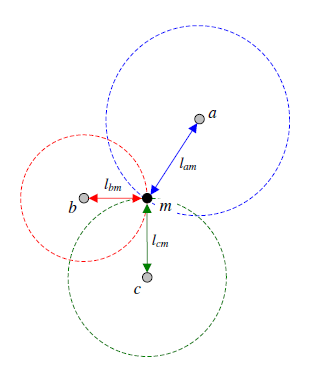
\includegraphics[resolution=300,width=0.39\textwidth,natwidth=610,natheight=642]{images/trilateracao.png}
    \caption{Esquema de Trilateração.}
    \label{fig:trilateracao}
\end{figure}


\begin{figure*}[ht]
\centering
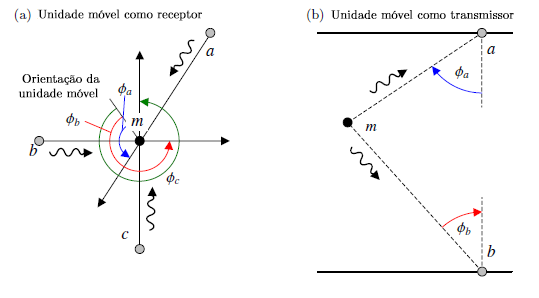
\includegraphics[resolution=300,width=0.65\textwidth,natwidth=610,natheight=642]{images/triangulacao.png}
    \caption{Esquemas de triangulação.}
    \label{fig:triang}
\end{figure*}

\subsubsection{Triangulação}\label{sec:triang}


A localização baseada na trilateração implica que os participantes devem ser capazes de medir distâncias (ou diferenças de distância) entre si. A triangulação funciona de forma semelhante, mas em vez de distâncias, os ângulos são medidos. De fato, pode-se demonstrar que a triangulação pode ser transformada em trilateração por meios simples\cite{linde2006aspects}. 

Triangulação requer a medição de ângulos entre as unidades de referência fixas e o alvo móvel. As unidades móveis calculam os ângulos em direção aos sinais emitidos por unidades fixas de referência. Obtém-se então a posição e orientação através dos dados recolhidos. As unidades de referência medem os ângulos na direção do sinal emitido pela unidade móvel. Apenas uma estimativa da localização, mas não a orientação do alvo móvel, pode ser obtida \cite{lutzke2013experimental}. Dois casos podem ser distinguidos, conforme ilustrado na Figura~\ref{fig:triang}:


\begin{itemize}
  \item A unidade móvel mede os ângulos em direção a sinais emitidos por unidades de referência fixas (ver Fig.~\ref{fig:triang}(a)). Os dados recolhidos fornecem a posição e orientação.
  \item As unidades de referência medem ângulos em direção ao sinal emitido pela unidade móvel (ver Fig.~\ref{fig:triang}(b)). Apenas uma estimativa de localização, mas não a orientação do alvo móvel, pode ser obtida.
 \end{itemize}


\subsubsection{Proximidade e análise de cena}\label{sec:proximidade}
Outra abordagem de localização é a técnica de detecção de proximidade na qual a posição de um alvo é aproximada, selecionando a localização da unidade de referência mais próxima. Por conseguinte, não é necessário cálculo de localização. Alternativamente, se várias unidades de referência estão dentro do alcance, o baricentro entre estas unidades podem produzir uma melhor estimativa \cite{EHuber1996}.

Pontos de referência (\textit{Landmarks}) são elementos estáticos de um ambiente que pode ser reconhecido por uma unidade móvel. Na maioria das vezes, os pontos de referência são formas geométricas, como retângulos, linhas ou códigos de barras. Itens naturais, como portas podem também servir como pontos de referência. O termo  análise de cena é frequentemente utilizado neste contexto. Unidades móveis tentam localizar-se  em determinado ambiente usando a visão da câmera, bem como funcionalidades de extração para analisar o cenário atual. Uma vez que um marco foi reconhecido e identificado de forma confiável, a posição atual da unidade em relação ao marco correspondente pode ser calculada. Isto é conseguido através de triangulação, trilateração e proximidade \cite{linde2006aspects}.

Detecção e localização do ponto de referência faciais são muito importantes para auxiliar tarefas de reconhecimento e rastreamento facial e reconhecimento de expressão facial \cite{cceliktutan2013comparative}. Detectar os pontos de referência do rosto consiste em duas tarefas principais. O primeiro é a detecção de rosto. O objetivo desta tarefa é encontrar face(s) em uma imagem (se houver) e extrair sua localização (por exemplo, coordenadas). Uma abordagem popular é o Viola e Jones \textit{face detector} \cite{viola2001rapid,viola2004robust}. A segunda tarefa é a detecção de marcos faciais. O objetivo é extrair os componentes faciais, como olhos, sobrancelhas, nariz, narinas, boca e contorno facial de faces detectadas, colocando pontos de referência em cada componente \cite{zhang2010survey}.

 \subsection{Reconhecimento facial}\label{sec:recFacial}
O reconhecimento facial é uma forma de identificar pessoas. Em desenvolvimento há muitos anos. esses sistemas permitem identificar alguém a um longo alcance, porém limitado principalmente pela resolução da câmera utilizada. No entanto, esta solução vem com algumas desvantagens. A adição de vigilância para o vídeo é necessária e, mesmo que seja explicitamente afirmado que as imagens são processadas e não armazenadas, ainda suscita preocupações que podem causar desconforto a alguns usuários. Outra desvantagem é que o software de reconhecimento facial não é muito confiável quando se trata de identificar dois seres semelhantes, como irmãos gêmeos idênticos \cite{fitzpatrick2013real}.

O reconhecimento de faces e mais vantajoso nesse aspecto, pois é possível realizar a identificação de uma pessoa sem ela cooperar ou saber que está sendo identificado. Primeiro é necessário detectar e segmentar faces de cenas complexas (Detecção de Faces). Para cada face, o processo de extração de característica é aplicado (Extração de Característica) e as características extraídas são comparadas com os \textit{templates} cadastrados na galeria de faces. A decisão sobre a identidade da face é então tomada (Reconhecimento de face) \cite{cardia2015avaliaccao}.   
 
 \subsection{\textit{Kinect}}\label{sec:kinect}
 
O \textit{Kinect} (Fig.~\ref{fig:kinect}) é um sensor de movimento, projetado pela \textit{Microsoft Inc}. e lançado em novembro de 2010 para ser usado como controle remoto para o console de videogames Xbox 360. É composto por vários sensores (Fig. ~\ref{fig:kinect}): Uma câmera RGB (Color CMOS, VNA38209015), uma câmera de profundidade composta por um projetor de infravermelho (\textit{infrared} - IR) (OG12 / 0956 / D306 / JG05A) combinado a uma câmera de infravermelho (IR CMOS, \textit{Microsoft} / X853750001 / VCA379C7130) e uma série de quatro microfones. A câmera infravermelha e a câmera colorida têm uma definição de 640 x 480 \textit{pixels}. O ângulo de visão é $60\,^{\circ}$ horizontal e $45\,^{\circ}$ vertical. O dispositivo foi projetado para ser usado em uma faixa de 0,5 m a 5 m \cite{sevrin2015characterization}. A tabela \ref{table:comparativoScanners} apresenta um comparativo entre o \textit{Kinect} e os \textit{scanners} 3D mais utilizados.

 \begin{figure}[ht]
\centering
    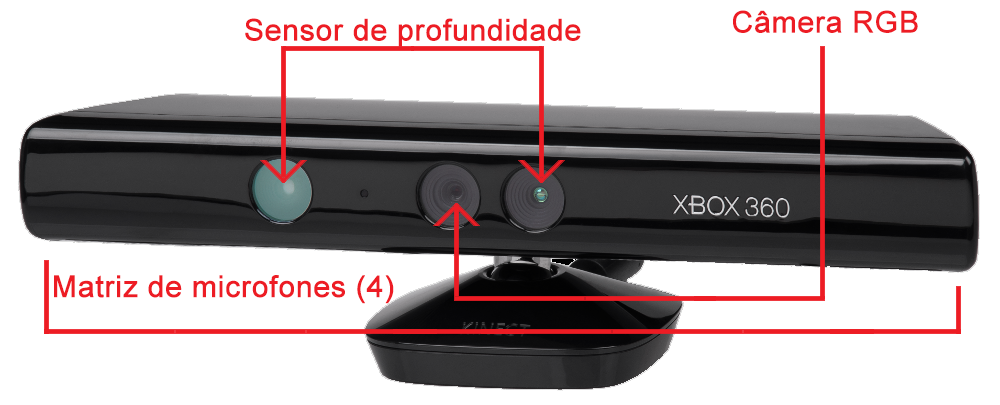
\includegraphics[resolution=300,width=0.4\textwidth,natwidth=610,natheight=642]{images/kinect.png}
    \caption{O Sensor \textit{Microsoft Kinect}.}
    \label{fig:kinect}
\end{figure}


 \begin{table}[ht]
 \caption{Comparação entre diferentes \textit{scanners} 3D \cite{li2013using}.\newline A velocidade é expressada em segundos, tamanho em polegadas, preço em USD e a acurácia é uma aproximação expressada em mm.}
 \label{table:comparativoScanners}
 \begin{tabular}{|l|c|c|c|c|c|}
\hline  
 Dispositivo & Velocidade & Carga & tamanho & Preço & Acurácia \\ \hline  
 3dmD & 0.002 & 10 s & N/A & >\$50k & <0.2 \\ \hline  
 Minolta & 2.5 & Não & 1408 & >\$50k & 0.1 \\ \hline  
 Artec Eva & 0.063 & Não & 160.8 & >\$20k & 0.5 \\ \hline  
 3D3 HDI R1 & 1.3 & Não & N/A & >\$10k & 0.3 \\ \hline  
 SwissRanger & 0.02 & Não & 17.53 & >\$5k & 10 \\ \hline  
 David SLS & 2.4 & Não & N/A & >\$2k & 0.5 \\ \hline  
 Kinect & 0.033 & Não & 41.25 & >\$200k & 1.5-50 \\ \hline
\end{tabular}
\end{table}


 \subsubsection{Câmera de profundidade (\textit{Depth-camera})}\label{sec:depth}
A câmera de profundidade é um dispositivo que pode detectar diretamente o alcance da superfície física mais próxima em cada pixel. A câmera de profundidade é única porque possibilita a modelagem 3D em tempo real da geometria da superfície. As câmeras de profundidade oferecem várias vantagens em relação aos sensores de intensidade tradicionais, trabalhando em baixos níveis de luz, fornecendo uma estimativa de escala calibrada, sendo invariante de cores e texturas e resolvendo ambiguidades de silhueta em pose. Eles também simplificam muito alguns difíceis problemas de visão computacional, como a remoção de fundo falso em uma aplicação de videoconferência \cite{wilson2010combining}. Além disso, é capaz de sintetizar imagens de profundidade realistas de pessoas e, assim, criar um grande conjunto de dados de treinamento, com baixo custo. Algumas das tecnologias usadas para obter informações de profundidade da câmera em profundidade são luz infravermelha e estruturada de tempo de vôo (\textit{time-of-flight}) \cite{bogomjakov2006free}.

O trabalho de Jamie Shotton et. al\cite{Shotton:2013:RHP:2398356.2398381} emprega simples recursos de comparação de profundidade, inspirados por aqueles em \cite{lepetit2005randomized}. Em um dado pixel $x$, a funcionalidade computa: 

\begin{align}
{f_{\theta}}(I, x) = d_{I}  \left(x + \frac{\boldsymbol{u}}{d_{I}(x)}\right) -  d_{I} \left(x + \frac{\boldsymbol{v}}{d_{I}(x)}\right) ,
\label{eq:eq1}
\end{align}

Onde $d_{I}(x)$ é a profundidade do pixel $x$ na imagem $I$ e os parâmetros $\theta = (\boldsymbol{u,v})$ descreve os \textit{offsets} $\boldsymbol{u}$ e $\boldsymbol{v}$. A normalização dos \textit{offsets} por $\frac{1}{d_{I}(x)}$ garante que os recursos sejam invariantes de profundidade: em um determinado ponto do corpo, um deslocamento de espaço fixo resultará se o pixel está próximo ou longe da câmera. Os recursos são, portanto, invariantes de translação 3D (efeitos de perspectiva de módulo). Se um \textit{pixel} deslocado estiver no fundo ou fora dos limites da imagem, a sonda de profundidade $d_{I}(x')$ recebe um grande valor constante positivo.




\subsubsection{Nuvem de pontos (\textit{Depth-camera})}\label{sec:nuvem}
A nuvem de pontos é uma estrutura de dados usada para representar uma coleção de pontos multi-dimensionais e é comumente usada para representar dados tridimensionais. Em uma nuvem de pontos 3D, os pontos geralmente representam as coordenadas geométricas $X$, $Y$ e $Z$ de uma superfície subjacente amostrada. Quando as informações de cor estão presentes, a nuvem torna-se ponto 4D \cite{gustavo2014Localizacao}.

\subsubsection{Triangulação estéreo }\label{sec:steroTriang}
Triangulação estéreo é um algoritmo de análise para calcular a posição 3D de pontos em um quadro de imagem. Em geral, triangulação estéreo, duas imagens são usadas para obter as duas visualizações diferentes em uma cena, de forma semelhante à visão binocular humana. Ao comparar essas duas imagens, a informação de profundidade relativa é calculada \cite{kinect4Windows}. 

\subsubsection{Inferência de partes do corpo e sugestão de \textit{joints}}\label{sec:bodyProposal}

Uma contribuição fundamental do trabalho realizado pela \textit{Microsoft} \cite{Shotton:2013:RHP:2398356.2398381} no desenvolvimento do \textit{Kinect} SDK é a representação parcial de partes do corpo. São Definidos vários rótulos de partes localizadas de um individuo, que cobrem densamente o corpo, como codificado por cores na Figura \ref{fig:bodyparts}. Algumas dessas partes são definidas para localizar diretamente as articulações esqueléticas de interesse, enquanto outras preenchem as lacunas ou podem ser usadas em combinação para prever outras articulações.

As partes são especificadas em um mapa de textura que é retornado para diminuir os vários caracteres durante a renderização. Os pares de imagem e profundidade da parte do corpo são usados como dados totalmente rotulados
para o aprendizado do algoritmo classificador. Para os experimentos foram usadas 31 partes do corpo (E-Esquerda, D-Direita, S-Superior, I-Inferior): cabeça (ES, DS, EI, DI), pescoço, ombro (E, D), braço (ES, DS, EI, DI),cotovelo (E, D), pulso (E, D), mão (E, D), torso (ES, DS, EI, DI), perna (ES, DS, EI, DI), joelho (E, D), tornozelo (E, D) e pé (E, D). Partes distintas para esquerda e direita permitem ao classificador desambiguar os lados esquerdo e direito do corpo \cite{Shotton:2013:RHP:2398356.2398381}.

\paragraph{Florestas de decisão aleatória }\label{sec:forests}

As árvores e florestas de decisão aleatória \cite{quinlan1986induction, shepherd1983appraisal, amit1997shape, breiman2001random} demonstraram classificações rápidas e eficazes para várias tarefas \cite{lepetit2005randomized, moosmann2007fast, shotton2008semantic}, e podem ser implementadas de forma eficiente na GPU \cite{sharp2008implementing}. Conforme ilustrado na figura \ref{fig:decisionTree}, uma floresta é um conjunto de árvores de decisão $T$, cada uma constituída por nós de divisão e folhas. Cada nó dividido consiste em uma característica ${f_{\theta}}$ e um limite $\tau$. Para classificar o pixel $x$ na imagem $I$, um começa na raiz e avalia repetidamente a equação \ref{eq:eq1}, ramificando para a esquerda ou para a direita de acordo com a comparação com o limite $\tau$. No nó da folha alcançado na árvore $t$, uma distribuição aprendida $P_{t} (c | I, x)$ sobre as etiquetas das partes do corpo $c$ é armazenada. As distribuições são calculadas em média para todas as árvores na floresta para dar a classificação final.

\begin{align}
P(c | I, x) = \frac{1}{T} \sum_{t=1}^{T} P_{t} (c | I, x).
\label{eq:eq2}
\end{align}

Cada árvore é treinada em um conjunto diferente de imagens sintetizadas aleatoriamente. Um subconjunto aleatório de 2000 exemplos de \textit{pixels} de cada imagem é escolhido para assegurar uma distribuição aproximadamente igual em partes do corpo. Cada árvore é treinada usando o seguinte algoritmo: 

\begin{enumerate}
    \item Propor aleatoriamente um conjunto de candidatos divididos $\phi = ({\theta}, \tau)$ (Caracterizar os parâmetros $\theta$ e os limiares $\tau$ );
    \item Particionar o conjunto de exemplos $Q = \{(I, x)\}$ nos subconjuntos esquerdo e direito por cada $\phi$:
    
        \begin{align}
            Q_{1}(\phi) = \{\,(I, x)\,|\, {f_{\theta}}(I, x) < \tau\,\} \\
            Q_{r}(\phi) = Q\, \textbackslash \,Q_{1}(\phi) \MoveEqLeft[5.1] 
            \label{eq:eq3_4}
        \end{align}
    \item Calcule o $\phi$ Dando o maior ganho de informação:
    \begin{align}
            \phi^* &= \operatornamewithlimits{argmax}_\phi G(\phi) \\
             G(\phi) &= H(Q) - \sum_{s\in \{1,r\}} \frac{|Q_{s}(\phi)|}{|Q|}H(Q_{s}(\phi))
            \label{eq:eq5_6}
        \end{align}
        Onde a entropia de Shannon\footnote{A entropia é definida como sendo uma forma de medir o grau médio de incerteza a respeito de fontes de informação, o que consequentemente permite a quantificação da informação presente que flui no sistema. Em termos simples, o conceito de entropia se associa à ideia de que, quanto mais incerto é o resultado de um experimento aleatório, maior é a informação que se obtém ao observar a sua ocorrência.} \cite{shannon2001mathematical}
$H(Q)$ é calculada no histograma normalizado das etiquetas das partes do corpo $l_{I}(x)$ para todos $(I,x) \in Q$.
    \item Se o maior ganho $G(\phi^{*})$ for suficiente e a profundidade na árvore estiver abaixo de um máximo, então recolete para subconjuntos esquerdo e direito $Q_{1}(\phi^{*})$ e $Q_{r}(\phi^{*})$.
\end{enumerate}

Para manter os tempos de treinamento baixos, foi empregada uma implementação distribuída. Treinar três árvores com profundidade tamanho 20 em um milhão de imagens leva cerca de um dia em um \textit{cluster} de mil núcleos.

\begin{figure}[ht]
\centering
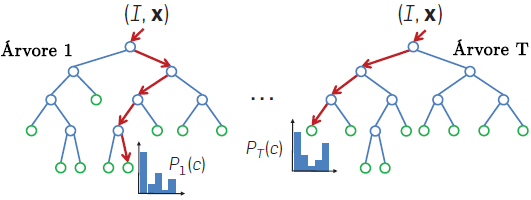
\includegraphics[resolution=300,width=0.45\textwidth,natwidth=610,natheight=642]{images/tree_decision.png}
    \caption{\textbf{Florestas de decisão aleatória}. Uma floresta é um conjunto de árvores. Cada árvore consiste em nós divididos (azul) e nós folha (verde). As setas vermelhas indicam os caminhos diferentes que podem ser tomadas por árvores diferentes para uma entrada específica \cite{Shotton:2013:RHP:2398356.2398381}.}
    \label{fig:decisionTree}
\end{figure}

\begin{figure*}[ht]
\centering
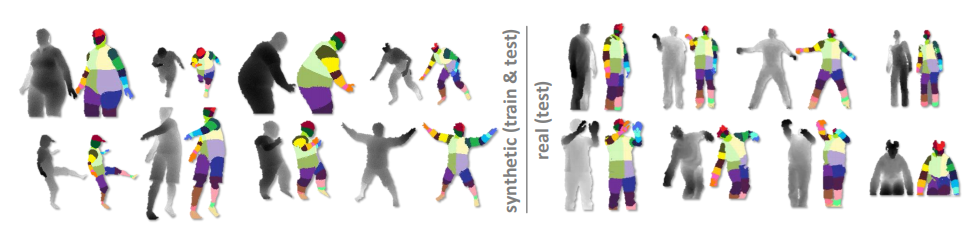
\includegraphics[resolution=300,width=1.0\textwidth,natwidth=610,natheight=642]{images/body_parts.png}
    \caption{Dados sintéticos e reais. Pares de imagens de profundidade e partes verdadeiras do corpo, com grande variedade de pose, forma, roupa e cortes \cite{Shotton:2013:RHP:2398356.2398381}.}
    \label{fig:bodyparts}
\end{figure*}


Este trabalho, utiliza uma recente abordagem sensorial: a utilização de mapas de profundidade para a detecção de presença em um ambiente interno. Tratando-se de um sistema biométrico, do tipo físico, tendo como características desse tipo de sistema: não cooperativa, sigilosa, não habituado, não auxiliado e \textit{less intrusive}. o \textit{Kinect SDK} utiliza os resultados do algoritmo de florestas de decisão aleatória para identificar \textit{joints} e partes do corpo de indivíduos em uma cena. A partir de tecnologias visuais, livre de marcador, são utilizados processos de triangulação estéreo para extração do mapa de profundidade, calculando a partir desse, a posição física dos indivíduos.
\section{Trabalhos Relacionados}\label{sec:trabalhos-relacionados}

A pesquisa sobre o monitoramento de vídeo dinâmico tornou-se mais madura nos últimos anos. Na literatura especializada, o conjunto de trabalhos que utilizam dados do
\textit{Microsoft Kinect} para o reconhecimento BD de faces é bastante reduzido. Os trabalhos mais interessantes são os de Goswami et al. \cite{goswami2013rgb} e Li et al. \cite{li2013using}.

Goswami et al. \cite{goswami2013rgb} geram mapas de entropia e saliência visual para os dados gerados pelo \textit{Kinect}. Para as imagens RGB ambos os mapas são gerados, para os dados de profundidade somente o mapa de entropia é gerado. O descritor da face é gerado concatenando os HOGs (Histograma de Gradientes Orientados) de diferentes fragmentos de ambos os mapas. Para a classificação dos sujeitos e utilizado o Classificador RDF (Floresta Randômica de Decisão).
 
Li et al. \cite{goswami2013rgb} também utilizam tanto os dados de profundidade quanto as imagens RGB para fazer detecção 3D de faces. Como primeiro passo do método os dados em RGB passam pela transformada DCS (Espaço de Cor Discriminante) para aumentar seu poder discriminativo. Como possuem três canais eles são empilhados. As imagens de profundidade são baseadas nas nuvens de pontos gerada pelo  \textit{Kinect}. Para melhorar a densidade elas são submetidas a um processo de Preenchimento Simétrico ( \textit{Symmetric Filling} no original).
 
Preenchimento Simétrico e um processo onde a nuvem de pontos de uma face é espelhada e, cada ponto na face original, é comparado com um ponto na nuvem espelhada. Caso a distância entre os dois pontos seja menor que um  \textit{threshold t} então o ponto da nuvem espelhada passa a fazer parte da nuvem original. Devido às propriedades simétricas da face esse processo tende a melhorar a qualidade dos dados gerados pelo \textit{Kinect}.
 
Após gerar as imagens de profundidade baseadas nas novas nuvens de pontos o classificador SRC (Classificador de Representação Esparsa) é utilizado para classificação dos sujeitos.
 
Mandeljc et al. \cite{mandeljc2012tracking} propuseram um sistema usando Banda ultralarga (\textit{Ultra wideband - UWB}) e vídeo para o posicionamento de pessoas em ambientes \textit{indoor}. Embora este sistema tenha um bom efeito de posicionamento, equipamentos UWB e múltiplas câmeras são obrigados a ser instalado no local, tornando o custo de construção do sistema é muito alto.

Wang et al. \cite{wang2011flexible,wang2011rfid} criaram um sistema de monitoramento em tempo real e posicionamento de pessoas em ambientes \textit{indoor} combinando imagem com  tecnologias RFID. No entanto, encontra-se experimental e continuam a verificar sobreposição de pessoas e problemas de blindagem, bem como os resultados de posicionamento são susceptíveis de serem influenciadas por altura e tipo do corpo, assim, o efeito implementação requer melhorias.

A utilização do \textit{Kinect} resolve os problemas anteriormente referidos. Com o \textit{Kinect} pode-se extrair com precisão as pessoas e a identificação não terá falhas resultantes de diferentes alturas, tipos de corpo e cores de pele. Seu o chip de processamento de imagem incorporado pode aumentar significativamente a eficiência do processamento de imagem, o que a torna muito aplicável à implementação de um sistema de posicionamento de pessoas \textit{indoor}.

Alguns estudos utilizam o \textit{Kinect} para projetar sistemas de posicionamento de pessoas. Schindhelm \cite{schindhelm2012evaluating} mostrou que o \textit{Kinect} foi muito aplicável no posicionamento \textit{indoor} de edifícios públicos. Nakano et al. \cite{nakano2012kinect} também propôs usar o \textit{Kinect} para o posicionamento de pessoas \textit{indoor}. No entanto, os sistemas acima referidos não têm a função de identificação de pessoas. 

Sung et al. \cite{sung2012unstructured} propõe um sistema de detecção de atividade e reconhecimento usando um sensor de RGBD \textit{Kinect}. Primeiramente é capturada a natureza hierárquica usando um modelo gráfico probabilístico hierárquico, especificamente modelo de entropia máxima de Markov (\textit{maximum entropy Markov model } - Memm) de duas camadas. Mesmo com esse modelo estruturado no lugar, pessoas diferentes realizam diferentes tarefas em velocidades diferentes, e qualquer modelo gráfico único, provavelmente, não consegue captar essa variação. Para superar esse problema, é apresentado um método de seleção de estrutura gráfica \textit{on-the-fly} que pode se adaptar a variações na velocidade automaticamente. O ultimo passo, para capturar as características significativas de uma pessoa, é utilizando o sistema de rastreamento de esqueleto \textit{PrimeSense} \cite{primeSence2014} em combinação com histograma de gradientes orientados. Esse trabalho tem seu foco, porém, na detecção de pessoas para extração de informações de atividades rotineiras de um certo indivíduo.


Há um grande corpo de outros trabalhos sobre o reconhecimento de atividade humana. Uma abordagem comum é usar características espaço-temporais para modelar pontos de interesse em vídeo \cite{dollar2005behavior,laptev2003space}.



Lu Xia et al. \cite{xia2011human} apresentam um método baseado em modelo para detecção humana a partir de imagens de profundidade. este método detecta as pessoas usando informações de profundidade obtidas pelo \textit{Kinect} em ambientes internos. utilizando um processo de detecção de cabeça de 2 estágios, que inclui um detector de borda 2D e um detector de forma 3D para então utilizar as informações de borda e as informações de mudança de profundidade relacional na imagem de profundidade. Também propõe um método de segmentação para segmentar a figura dos objetos de fundo que lhe são anexados e extrair o contorno geral do assunto com precisão. O método é avaliado em um conjunto de dados 3D previamente obtido pelo \textit{Kinect}.



A maior semelhança entre esse trabalho e os descritos anteriormente é que todos utilizam o \textit{Kinect} como um dispositivo substituto dos \textit{scanners} 3D tradicionais. Porém, ao contrário dos demais, este não utiliza as imagens RGB. Além disso, os trabalhos citados apenas executam um algoritmo de decisão sobre uma base de dados contendo imagens de mapas de profundidade gerados pelo  \textit{Kinect}, enquanto o objetivo desse trabalho é executar e exibir em  \textit{runtime} o resultado do algoritmo de detecção.

\section{Solução desenvolvida}\label{sec:solucao-desenvolvida}

\begin{figure*}[ht]
\centering
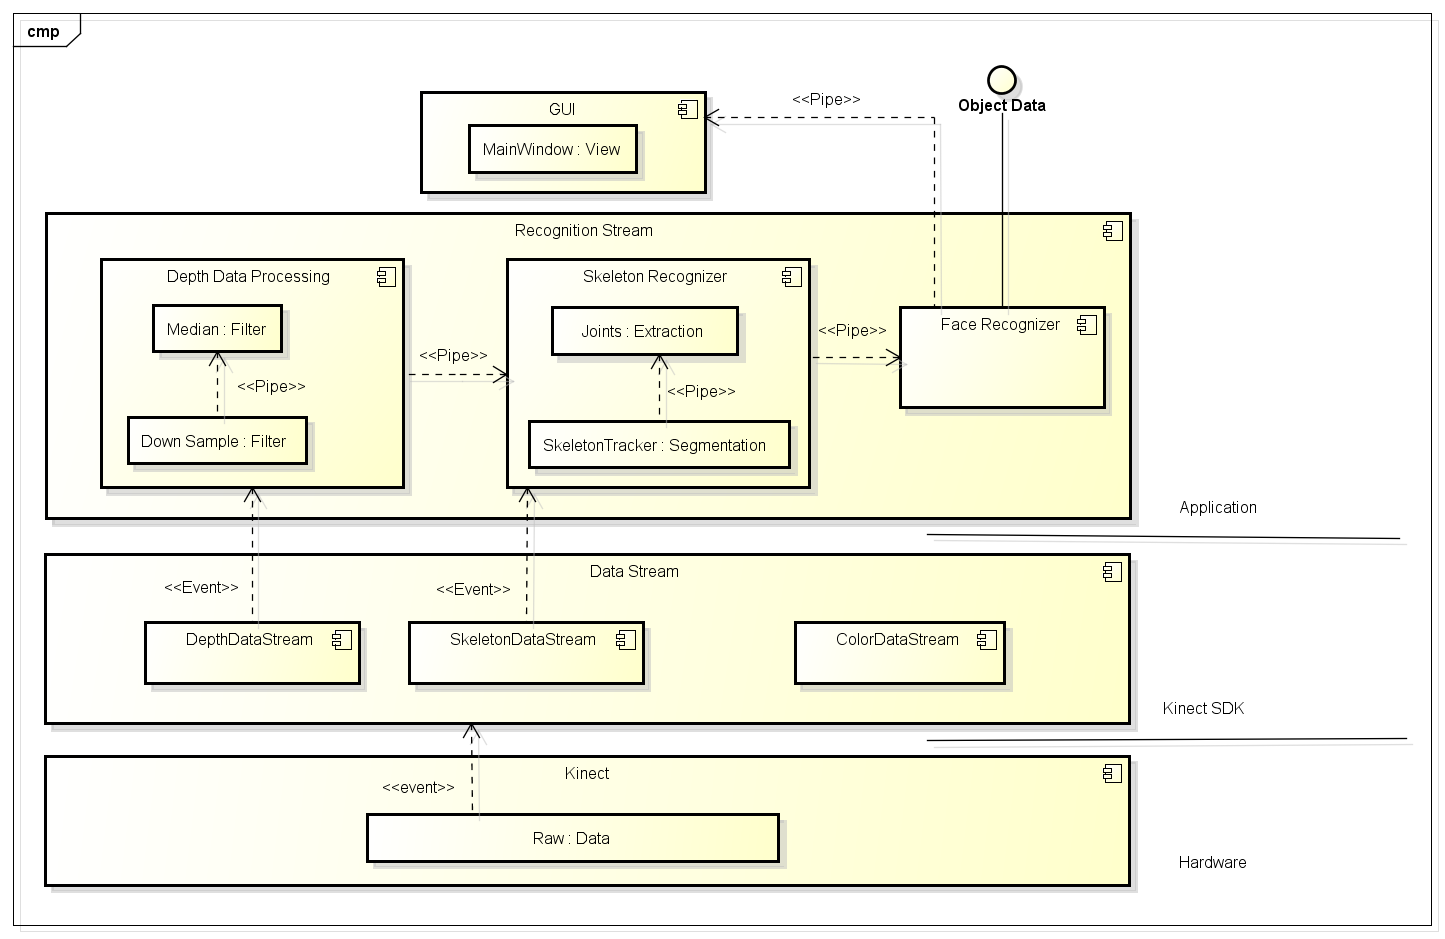
\includegraphics[width=1.0\textwidth]{images/Arquitetura_da_solucao.png}
\caption{Arquitetura da solução proposta}
\label{fig:visao-geral}
\end{figure*}

Motivado pela demanda de serviços de identificação de pessoas e pelo fato de que as soluções para tal problema ainda permanecem em aberto, este trabalho propõe a utilização de mapas de profundidade. O mecanismo de identificação consiste em extrair esse mapa através do projetor infravermelho e do sensor monocromático, e analisar os dados obtidos, utilizando de filtros e algoritmos de segmentação. Por fim, é exibida graficamente uma visualização do mapa de profundidade gerado e, em caso de positivo, o(s) indivíduo(s) encontrado(s) na cena. É exibido também os dados que podem ser exportados para plataformas externas: a localização aproximada dos sujeitos no plano 3D (posições $X$, $Y$ e $Z$) e a distância em relação ao \textit{Kinect}. Nesta seção é discutida a solução desenvolvida.

\subsection{Arquitetura da solução}\label{sec:arqSol}
Para processar os dados de profundidade do sensor \textit{Kinect}, a aplicação executa o seguinte fluxo de dados:

\begin{enumerate}
    \item Habilitar o canal de fluxo de profundidade com o tipo de formato de imagem em profundidade; 
    \item Anexar o manipulador de eventos ao canal de fluxo; 
    \item Processar os quadros de profundidade de entrada; 
    \item Renderizar os quadros na UI.
\end{enumerate}

O \textit{Kinect} é o responsável por obter a visualização da cena de um ambiente interno. Como discutido na seção \ref{sec:trabalhos-relacionados}, o \textit{Kinect} é um sensor de movimento muito eficiente, extraindo com precisão objetos, pessoas e detalhes de uma cena. A \textit{Microsoft} provê para o \textit{Kinect} um Kit de desenvolvimento de software (\textit{Software Development Kit}, SDK). O sistema é composto por módulos adicionados à camada de aplicação, Sobre a camada do SDK. A Figura \ref{fig:visao-geral} apresenta uma visão geral da solução.

\subsubsection{Estilos arquiteturais}\label{sec:estilosArq}
A solução apresenta um estilo arquitetural híbrido, com características de três estilos arquiteturais básicos:

\begin{itemize}
\item Baseado em invocação implícita: \textit{Event Based}; 
\item Baseado em fluxo de dados: \textit{Pipe and Filter}; 
\item Em camadas: \textit{Virtual Machine}.
\end{itemize}

O estilo baseado em eventos (\textit{Event Based}) é um estilo arquitetônico baseado na invocação implícita que fornece uma interação indireta entre componentes acoplados de forma livre, facilitando a adaptação e melhorando a escalabilidade do sistema. Os componentes do tipo de evento (\textit{Depth}, \textit{color} e \textit{Infrared}.) comunicam-se apenas através de eventos transmitidos por um conector de evento.
Este conector então retransmite os eventos para todos os componentes do tipo \textit{Observer} mostrando interesse no evento em questão (Nesse caso, o \textit{Recognition Stream}), melhorando assim a eficiência da distribuição de eventos.

\textit{Pipes} e Filtros (\textit{Pipe and Filter}) é um estilo arquitetural composto por uma cadeia de elementos de processamento, dispostos de forma tal que a saída de cada elemento é a entrada do próximo. O fluxo de dados se dá através de \textit{pipes} (canos) e os dados sofrem transformações quando processados nos filtros. Em outras palavras, os \textit{pipes} é que possibilitam o fluxo dos dados, e os filtros fazem o processamento dos mesmos, colocando-os nos \textit{pipes} antes que todos os dados de entrada sejam consumidos. Portanto, a nível de arquitetura, o processamento é mapeado em filtros e os \textit{pipes} agem como condutores de dados. O componente \textit{Recognition Stream} é composto por subcomponentes do tipo \textit{Filter} e a comunicação entre os mesmos se dá através dos conectores do tipo \textit{Pipe}. 

As arquiteturas de máquinas virtuais (\textit{Virtual Machines}) têm como objetivo alcançar a qualidade da portabilidade. Este estilo de arquitetural simula algumas funcionalidades que não são originais para o \textit{hardware} e/ou \textit{software} em que é implementado. O estilo é aplicado entre o \textit{Kinect (hardware)} e a aplicação desenvolvida, usando conectores do tipo \textit{Event} e \textit{Pipe} entre as camadas. Esse estilo arquitetônico reduz a complexidade, melhora a modularidade, reutilização e manutenção.
Conforme visto na figura \ref{fig:visao-geral}, o sistema possui as camadas:

\begin{itemize}
\item \textit{Kinect (hardware)};
\item \textit{Kinect} SDK; 
\item Aplicação; 
\end{itemize}

\subsubsection{Arquitetura do \textit{Kinect for Windows} SDK}\label{sec:kinectSDK}
O SDK fornece uma biblioteca e ferramentas de software sofisticadas para ajudar os desenvolvedores a usar a forma rica de entrada natural baseada no uso do \textit{Kinect}, que detecta e reage a eventos do mundo real. O \textit{Kinect} e a biblioteca de software interagem com aplicações, como mostrado na Figura \ref{fig:sdk_interact}. Os componentes do SDK são exibidos na figura \ref{fig:sdk_architecture_color} e incluem:

\begin{figure}[h]
\centering
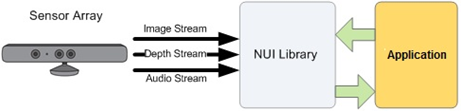
\includegraphics[width=0.5\textwidth]{images/sdk_interaction.png}
\caption{Interação de Hardware e Software com a Aplicação}
\label{fig:sdk_interact}
\end{figure}



\begin{enumerate}
    \item \textit{Hardware Kinect} - Os componentes de \textit{hardware}, incluindo o sensor \textit{Kinect} e o \textit{hub} USB através dos quais o sensor \textit{Kinect} está conectado ao computador;
    \item \textit{Drivers Kinect} - Os \textit{drivers} do Windows para o \textit{Kinect}, que são instalados como parte do processo de configuração do SDK. Os \textit{drivers} do \textit{Kinect} suportam:
        \begin{itemize}
            \item A matriz de microfones como um dispositivo de áudio em modo \textit{kernel} que pode ser acessado  através das API de áudio padrão no Windows; 
            \item Controles de transmissão de áudio e vídeo para transmissão de áudio e vídeo (cor, profundidade e esqueleto);
            \item Funções de enumeração de dispositivos que permitem que um aplicativo use mais de um \textit{Kinect}.	
        \end{itemize} 
    \item Componentes de Áudio e Vídeo:
        \begin{itemize}
            \item Interface de usuário natural do Kinect para rastreamento de esqueleto, áudio e imagem em cores e profundidade. 
        \end{itemize}
    \item Objeto de mídia DirectX (DMO) para formatação de feixes de microfone e localização de fonte de áudio;
    \item API padrão do Windows - APIs de áudio, voz e mídia no Windows, conforme descrito no SDK do Windows e no Microsoft \textit{Speech} SDK.
\end{enumerate}


\subsection{Componentes principais}\label{sec:componentes}

\subsubsection{Color Data Stream}\label{sec:colorDataStream}

\subsubsection{Depth Data Stream}\label{sec:depthDataStream}
\textcolor{red}{capturing data stream}

Quando se trata do Kinect, há apenas uma imagem, que é capturada pelo sensor de profundidade IR. Então, como funciona a triangulação estéreo? Na verdade, existem duas imagens em vez de uma. A segunda imagem é invisível - é um padrão do emissor IR, já definido com o laser IR. O laser IR não é modulado. Tudo o que o laser faz é projetar um padrão pseudo-aleatório de especificações no ambiente Kinect. Essas duas imagens não são equivalentes, pois há alguma distância entre o emissor IR e o sensor de profundidade IR. Essas duas imagens são consideradas como correspondência para diferentes câmeras e permitem a aplicação de triangulação estéreo para calcular a profundidade como mostrado na imagem \ref{fig:trilatStereo}. Essa imagem demonstra como $x1$ e $x2$ são medidos usando a triangulação estéreo para um ponto $X$ na cena.

\begin{figure}[!h]
\centering
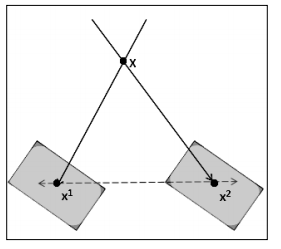
\includegraphics[width=0.4\textwidth]{images/trilateracao_estereo.png}
\caption{Trilateração estéreo para cálculo de profundidade.}
\label{fig:trilatStereo}
\end{figure}

o \textit{Depth Data Stream} lê os pontos na cena, processa os dados e envia a informação de profundidade a partir da qual eles foram refletidos, para o \textit{Recognition Stream}. Nele, é identificado o sensor \textit{Kinect} conectado e é ativado o canal do fluxo de profundidade:

\begin{minted}{csharp}
this.sensor = KinectSensor.KinectSensors[0];
this.sensor.DepthStream.Enable(
  DepthImageFormat.Resolution640x480Fps30);
\end{minted}

A classe \textit{ImageStream} possui o método \textit{Enable()} sobrecarregado. Por padrão, o sensor permite o fluxo de profundidade com o formato de imagem de profundidade de resolução 640x480 \textit{pixels} e 30 frames por segundo (\textit{Resolution640x480Fps30}).

Uma vez que o sensor é identificado e o fluxo de profundidade está habilitado, é anexado o manipulador de eventos \textit{DepthFrameReady} a um evento que é gerado cada vez que um novo \textit{frame} de profundidade está disponível:

\begin{minted}{csharp}
sensor.DepthFrameReady +=
  new EventHandler
  <DepthImageFrameReadyEventArgs>
    (sensor_DepthFrameReady);
\end{minted}


\begin{figure*}[ht]
\centering
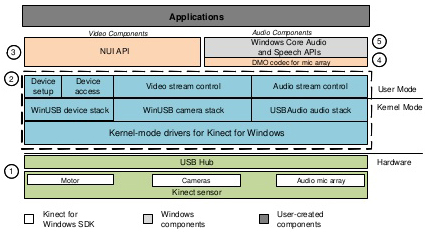
\includegraphics[width=0.8\textwidth]{images/sdk_architecture_color.png}
\caption{Arquitetura do SDK}
\label{fig:sdk_architecture_color}
\end{figure*}

\subsubsection{Skeleton recognizer }\label{sec:skeleton}
processing joints

\subsubsection{Depth Data Processing (Recognition Stream - Filter)}\label{sec:depthDataProcessing}
\textcolor{red}{processing data stream}
O manipulador de eventos \textit{DepthFrameReady} invoca com \textit{DepthImageFrameReadyEventArgs}, que possui o método \textit{OpenDepthImageFrame()} para retornar o quadro de imagem de profundidade atual enviado pelo sensor. O  método padrão para \textit{DepthFrameReady} é o \textit{SensorDepthFrameReady}. Nesse método, é recuperado o quadro de imagem em profundidade, usando o método \textit{OpenDepthImageFrame ()}, o qual retorna os dados de profundidade brutos do sensor. \textit{PixelData} cria o tamanho do \textit{buffer} para o quadro de imagem de profundidade de entrada.

O \textit{frame} de profundidade possui propriedades semelhantes que copiam os dados de \textit{pixels} para o \textit{buffer} recém-criado. \textit{CopyPixelDataTo()} é usado para copiar o \textit{array} de bytes de dados de \textit{pixels} do quadro de imagem atualmente recebido para o \textit{buffer}. Antes de copiar os dados de \textit{pixels}, primeiro é calculado o tamanho do \textit{buffer} usando a propriedade \textit{PixelDataLength} e, em seguida, é copiada a mesma imagem do \textit{array} de bytes como \textit{DepthImageFrame}. Como o quadro bruto de imagem de profundidade é uma imagem em escala de cinza de 16 \textit{bits}, \textit{PixelFormats} é especificado  como \textit{Gray16} ao criar a fonte de \textit{bitmap} para o controle de imagem em profundidade.

\textcolor{red}{adicionar aqui os metodos de filtro e segmentação...}
Finalmente, é criado o objeto \textit{BitmapSource} e atribuído ao controle de imagem \textit{depthImageControl}, que está definido no arquivo XAML para exibir os dados do fluxo.




\subsubsection{Face Recognition (Recognition Stream )}\label{sec:depthDataRecognition}
processing data stream
%\section{Avaliação Experimental}\label{sec:avaliacao-experimental}

Esta seção existe apenas no TCC. Ela não deve existir no pré-projeto.

Aqui será apresentado a estudo de avaliação conduzido para valiar a solução desenvolvida.
\section{Métodos e Materiais}\label{sec:metodos-e-materiais}


Será realizado um estudo de caso, baseado em pesquisa experimental pois há um alto nível de controle da situação e podem-se isolar todas as estruturas de qualquer interferência do meio exterior, gerando maior confiabilidade nos resultados.

Será realizada uma análise quantitativa da quantidade de coincidências entre trilhas e detecções de forma a avaliar e validar a eficiência em relação à detecção de falsos positivos indicados pela solução. Esses dados serão obtidos fazendo um comparativo entre o cenário real e os dados indicados pela solução. Será utilizada para isso a técnica de estudo experimental \textit{In Virtuo}

A avaliação se dará no que segue:

\begin{enumerate}
\item Adicionar o Kinect e os sensores em pontos estratégicos da sala;
\item Iniciar o sistema produto da solução;
\item Avaliar entrada e saída de um grupo distinto de pessoas em momentos distintos e ao mesmo tempo;
\item Comparar os dados obtidos pela solução com o ocorrido nas cenas durante a avaliação
\item Calcular a eficiência de acordo com os dados obtidos dessa comparação.
\end{enumerate}


%\subsection{Passo a Passo Latex}\label{sec:passo-a-passo}
Esta subseção apresenta o passo a passo que deve ser seguido para utilizar o sharelatex com o template da ECDU.

\begin{enumerate}
\item Criar projeto no ShareLatex com template IEEE Conference
\item Coloque as suas bibliografias em um arquivo separado. Para isso crie o arquivo .bib. Veja exemplo "\\bibliography{references.bib}
\\bibliographystyle{IEEEtran}" no texto. Remova a parte de referencias que já vem no template
\item No lugar dos dois itens anteriores, você pode fazer o download do projeto ECDU-TCC-Modelo e depois fazer o upload para sua conta, ou fazer a cópia direta (Opção Copy Project no menu esquerdo superior).
\item Mudar para português. Veja o código necessário aqui https://pt.sharelatex.com/learn/Portuguese. Esse código já está disponível no arquivo main.tex. Ele está entre os comentários "Início do código para entender português" e "Fim do código para entender português"
\item Corretor Ortográfico para português. Mude as configurações do seu projeto para Português do Brasil: Menu -> Spell Check -> Portuguese (Brazilian)
\end{enumerate}


\section{Conclusão}\label{sec:conclusao}

Sistemas e aplicações de localização interior tem experimentado nos últimos anos esforços adicionais com o aparecimento da computação ubíqua. Em vários cenários, objetos e pessoas precisam ser localizados ou monitorados. Por exemplo, em uma indústria ou ambiente médico. Além disso, a localização das pessoas viabiliza a criação de um grande número de aplicações e serviços. Clientes e funcionários podem ser observados, intrusos detectados, idosos suportados e pacientes monitorados. Em locais públicos, como estações de metrô, a segurança pode ser abordada por um sistema de orientação de emergência. Sistemas que utilizam as informações de orientação alimentada com o posicionamento dos seres humanos podem trabalhar de forma mais eficiente do que um sistema estático. 

O presente trabalho implementa um sistema que utiliza técnicas visuais com o objetivo de detectar pessoas em um ambiente fechado. Para tal, foi utilizado o \textit{Kinect} como sensor visual. A ferramenta desenvolvida utiliza o mapa de profundidade gerado pelo sistema de câmeras do \textit{Kinect} aplicando sobre essa fonte de dados algoritmos de filtro e segmentação visando a correta identificação de indivíduos em determinado âmbito.
Com essas características, as principais contribuições são:

\begin{enumerate}
    \item Baixo custo de \textit{hardware}, se comparado o \textit{Kinect} com os principais \textit{scanners} 3D do mercado;  
    \item Exportação de dados de localização dos sujeitos dentro do ambiente monitorado para que plataformas externas possam consumí-los;
    \item Eficiência, se comparado com projetos de detecção que utilizam técnicas visuais 2D e abordagens híbridas;
    \item \textit{less intrusiveness}, pois apenas o mapa de profundidade é exibido, se compararmos com sistemas que utilizam câmeras RGB. 
\end{enumerate}

Sua estrutura arquitetural dividida em camadas e módulos, seguindo o estilo \textit{Pipe and Filter} permite a fácil alteração dos componentes, sem causar impacto nos outros  elementos da solução. 

\subsection{Limitações deste Trabalho}\label{sec:limitacoes}
Este trabalho não contempla a avaliação da velocidade nem direção/sentido ao qual pessoas se movimentam, limitando-se a identificar a posição do objeto de estudo num determinado ambiente.
Outra limitação refere-se ao limite de distância ao qual o \textit{Kinect} é capaz de identificar objetos e pessoas, pois a versão um do mesmo possui \textit{range} entre 0,8 e 4 metros. Ainda, uma outra limitação do hardware em uso é a quantidade máxima de seis pessoas a serem identificadas, por ambiente.

\subsection{Trabalhos Futuros}
Como trabalhos futuros, podem-se aplicar outras técnicas de processamento e detecção de pessoas, estimando e comparando o nível de eficácia da solução. Outra abordagem seria a adição de sensores não visuais, como por exemplo pisos táteis ou sensores ultrassônicos. Os dados exportados pela aplicação (distância e coordenadas) podem ser usados por uma grande variedade de sistemas, como por exemplo sistemas de segurança, \textit{home, baby e Elderly care}, industriais, entre outros. Utilizar esses dados em um sistema de visualização 3D é igualmente interessante.

Para as restrições do \textit{hardware} citados na subseção \ref{sec:limitacoes} pode-se tanto adicionar outros \textit{Kinects} quanto substituir o \textit{Kinect} V1 pela segunda versão do mesmo, melhorando assim a Acurácia, precisão e \textit{range} da solução.



%\appendices
%\section{Dicas de escrita}
\begin{enumerate}
\item Evitem textos grandes, com poucos pontos de continuação. Cada período deve conter uma única informação.
\item Evitem erros de gramática/ortografia. Isso é muito grave.
\item ll
\end{enumerate}


% use section* for acknowledgement
%\section*{Acknowledgment}

%Os autores deste trabalho gostariam de agradecer ao ...


% Can use something like this to put references on a page
% by themselves when using endfloat and the captionsoff option.
\ifCLASSOPTIONcaptionsoff
  \newpage
\fi


% biography section

\bibliography{references.bib}
\bibliographystyle{IEEEtran}


% that's all folks
\end{document}


